\documentclass[11pt, a4paper]{report}
\usepackage{appendix}
\usepackage{fullpage}
\usepackage{graphicx}
\usepackage{subcaption}

\DeclareGraphicsExtensions{.jpg, .png, .pdf} %.jpg .png .pdf
\renewcommand{\abstractname}{Executive Summary}

\setlength{\parskip}{0.3cm}
\setlength{\parindent}{0cm}

\begin{document}

\begin{titlepage}

\title{VisualHeap
\\A 3D Heap Visualiser for Object Oriented Programs}
\author{Aviv Beeri, Briony Goldsack, Ying Jiang,
\\Oliver Myerscough, Anna Thomas, Eleanor Vincent}
\maketitle

\end{titlepage}

\tableofcontents

\begin{abstract}
A deep understanding of programs is required to build the next wave of garbage collectors and explicit allocators. In order to facilitate such an understanding it is important that the foundation blocks of a developer’s learning are robust. As things are, there are currently very few tools present within the industry that allow a developer, or even simply an interested party, to deconstruct the information of their program’s heap in any meaningful way other than through the standard debuggers such as GDB or those provided in IDEs such as Eclipse or Intellij. These methods largely provide only a textual representation of the information  but this is often a poor way to represent the data structure of the program at any particular moment in the program’s lifetime. The data structures such as trees and graphs are very difficult for some programmers to grasp given the standard IDE debugging layout. 

An object-oriented software application creates complex structures on the heap during its lifetime. Debugging object-oriented software often involves thinking about how the heap evolves as a program runs. The aim of our group project is to design a tool which supports visualisation of the heap of a running Java program as a 3D scene which can be navigated by the software developer by moving around as if in a first person shooter game.

VisualHeap is a simple debugging program designed as a teaching aid to compliment first-year Java courses. Within the program the user is able to load different applications and view a 3D graphical representation of the structure of the code. The idea behind this is to aid those new to the language to understand the concepts behind object-oriented programming and see how the code they write affects the programs they create in a clear manner. Data visualisation has always been an interesting topic; this program aims to continue the trend to reinvent the way we, as developers, think about the application we create. With each new way the information can be presented, a new idea or solution can be more easily accessed. 

As a teaching aid, VisualHeap aims to help improve the intuitive reasoning of students with regards to understanding best practice for program structure and serves as a helpful first look into the art of debugging a program. VisualHeap is a very basic debugger, with only a handful of the features that exist within the industry. With this style of program a student can begin to see why the process is useful and start to build a workflow within this program before moving onto more complex debuggers with a wider range of features and larger pool of information.  VisualHeap aims to bridge that gap whilst giving a certain amount of visual interactivity between the developer and their code. 
\end{abstract}

\chapter{Introduction}
\section{What is the heap?}

The heap is memory set aside for dynamic allocation. Within Java, the heap, a runtime data area from which memory for class instantiation and arrays are allocated, is created at the start-up of the JVM. Whenever we create a new object it is allocated a block of memory from the heap; the memory is freed when the object is destroyed by the garbage collector.

\section{Motivation}

A strong motivation behind the VisualHeap project was as a teaching aid. When many people begin programming they do not know what the heap is in Java, or are even aware of where objects are created. Learning about the Java heap is a key part of understanding the language so you can deal with, for example, a java.lang.OutOfMemoryError and analyse heap dumps. We know learning the basics of programming can be a difficult process for many people as there is no formal process that can teach you everything you need to know. In the first year Java course at Imperial, and many other courses, the heap is described using a simple 2D diagram similar to the one shown below (Figure whatever). This is currently the main method of explaining how objects are created in the heap and how they reference each other. Whilst adequate for some, many would find alternative explanations of the concept useful to cement their understanding of the concepts. For the most part, these alternate visualisations are not readily available . A visualisation of the way in which the heap (arguably the most prominent feature of an OO language) is populated would be an invaluable tool. 

Being an interactive tool, VisualHeap has the potential to be more engaging than a simple diagram; a live demonstration breaks up the lecture. Students can pose questions and use the tool (either on their own time or in a lecture) to answer them. VisualHeap also represents a goal for first year students. It is an exciting program of reasonable size and the point can be made that they too could build a system like this after following the Java course.

Expanding on this teaching point, as technology develops more and more complex projects are being developed, increasing the complexity of the debugging process. Debugging in a traditional development environment can be tedious and challenging, and this is due to tools which are unintuitive for the task at hand. For example, trying to follow complex data structures (Trees, Graphs) in a debugging environment is quite messy when performed in an IDE such as Eclipse. Providing a simplified environment to those new to the concepts of debugging would help those who struggle to understand the need for such tool ease into the workflow. With a simple and clean layout VisualHeap would provide a useful setting to encourage further independent learning on the topic. 

To compliment this, throughout the world in many different industries in the world, data visualisation has always been a diverse and interesting area for exploration. Within technology there are many projects devoted to finding new ways to extract data and develop creative, intuitive solutions to the issues the industries faces. With respect to heap visualisation, and memory management in general, there are significantly fewer tools readily available; those that are tend to be either too specialised or are not especially innovative in presenting their data. VisualHeap aims to begin to challenge this and develop a more interesting, interactive mode in which to view broad variety of programs.

\section{Objectives}

VisualHeap is a tool to visualise the heap of a Java program in 3-dimensional space, for the purposes of teaching and debugging, that aims to address the issues discussed above. We have  outlined the key objectives and their targets (who they will benefit) below.

\begin{quote}

\begin{itemize}
  \item Students
\end{itemize}
Increase understanding what the heap is \\
How objects are created and stored \\
Understanding large data structures such as trees and graphs

\begin{itemize}
  \item Lecturers
\end{itemize}
Provide an alternative tool for teaching object-oriented languages

\begin{itemize}
  \item General Objectives
\end{itemize}
Provide an intuitive tool for debugging \\
Attractive and intuitive 3D visualisation of the heap of a Java program \\
Easy navigation and interactive objects \\
Intuitive and simple GUI to integrate with the Java program and run VisualHeap

\end{quote}

\section{Achievements}

VisualHeap is a suitable tool to accompany lecturers while teaching the first-year programming course by complementing the material and exercises. This is done by providing an interactive 3D visual representation of the example program allowing students to navigate their way through it’s heap.

Through an attractive and interactive 3D visualisation of the heap, students will be able to better understand and comprehend what the heap is. The ability to navigate the heap world should help increase understanding of how objects are connected to each other through references. Obtaining object information by interacting with the heap objects allows a student to discover more about the objects that live on the heap.

We have provided a simple debugging interface using the GUI, which can then provide a 3D representation of the heap at the click of a button to help analyse data structures and improve learning. We believe we have solved the problems stated above and more detail is provided about these solutions in later sections.

\chapter{Design}

\section{GUI}

Our project is intended for both students and teachers so it is important to provide an interface which makes our debugger easy to use. The tabbed interface presented when the user starts the program is intended to guide them through the workflow necessary for using any debugger:

\begin{enumerate}

  \item Choosing the program to debug
  \item Where in the program to breakpoint
  \item Running the program
  \item Encountering the breakpoint
  \item Visualising the results
  \item Stepping through the program or resuming until the program ends
  
\end{enumerate}

Any student new to debugging needs to learn these steps in order to use a debugger effectively on their own programs.

We consulted our project supervisor to help improve the usability of the GUI for a first time user, so some improvements have been made to make it more intuitive, however it is still not a perfect design. We would have liked to have tested with current first years, but their Java is not quite at the level where VisualHeap could be of use to them yet. 

\begin{figure}[h]
        \centering
        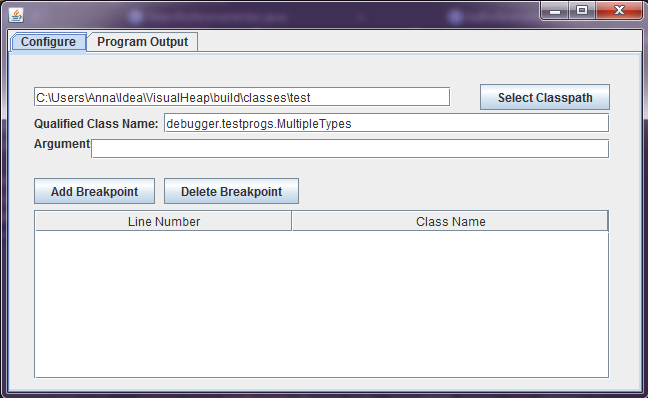
\includegraphics[width=0.75\textwidth]{images/final/gui.png}
        \caption{Program GUI}
\end{figure}

{\bfseries Heuristic Evaluation}: \\
In the absence of a key set of end users (first year students), we applied Nielsen’s heuristic evaluation for user interfaces.

{\bfseries Visibility of system status}: \\
By disabling buttons, setting cursor position, etc. we were able to improve the usability of the GUI bu guiding the user through the processes required to start the visualisation. Users should always be able to see what the state of the system is. We guide them by deativating fields for interactions that are inconsistent in the current state (i.e. the “Visualise” button is greyed out until the program is suspended at a breakpoint).

{\bfseries Match between system and the real world}: \\
The language used in the system should match the language of the real world. We use the normal terminology of debuggers. For advanced users this will be no problem, but those inexperienced with debuggers may not know the terms. An argument can be made that they should be introduced to these.

{\bfseries User control and freedom}: \\
There should be an “emergency exit”; users make mistakes and should not be penalised because of this. We have made sure breakpoints can be deleted.

{\bfseries Consistency and standards}: \\
Where there are standards and conventions, they should be followed. We have made sure we use the standard industry terminology in respect to both debuggers and the Java language.

{\bfseries Error prevention}: \\
A good design should preclude the possibility of errors occurring altogether. We have put validation upon inputs and defined a clear workflow. For example, the breakpoint controls are deactivated until a valid classpath and classname have been entered.

{\bfseries Recognition rather than recall}: \\
Users should not have to remember how the program is controlled; it should be immediately clear. We have made sure that no functionality is hidden away; the user can immediately see all the controls available to them.

{\bfseries Flexibility and efficiency of use}: \\
The system should include “accelerators” which provide experienced users with additional power. We have included command line arguments for prepopulating the classpath and target classname, along with setting a breakpoint.

{\bfseries Aesthetic and minimalist design}: \\
No irrelevant information should be presented to the user; this will compete with the relevant information for the user’s attention. We have split the GUI into two panes, one for setup (selecting a program, setting breakpoints) and another for running the program. This ensures that the user is focused on one task at a time.

{\bfseries Help users recognize, diagnose, and recover from errors}: \\
Error messages should be expressed in plain language, appropriate for users who do not know how the system works.

{\bfseries Help and documentation}: \\
It is best if a system can be used without documentation, but this is rarely the case.

\section{Exploring the 3D world}

\subsection{Movement}

Ensuring the heap is easily navigable was an important factor. As our graph is represented in the world on a 2D plane it is necessary that the user can gain a birds eye view to see the entirety of the graph. A user also needs to be able to interact with smaller objects which may require being closer to the ground. Due to these requirements we have granted the user the gift of flight. To give the user familiar controls we have attempted to make the movement as similar as possible to that of a first person shooter, with navigation being controlled by both customary keyboard controls and the mouse. 

\subsection{Object Representation}

We construct a graph of the heap with vertices representing objects and a directed edge between objects A and B iff one of A’s fields is a reference to B. We initially search to a depth of 3 references. Reference chains can be expanded further as the user desires. This dynamic approach is important as the heap of a Java program could be very large. Building the entire graph would be computationally intensive, and would lead to a very large and confusing representation.

The graph is rooted at the current stack frame. Visible variables in that frame make up the first level of objects to be presented. To improve clarity, we focus on the heap and ignore primitive types. We have defined 4 different kinds of vertices, representing each by different coloured 3D shapes. These are dummy vertices, object reference vertices, unfollowed reference vertices, and null reference vertices. How these map to implementation can be seen later in figure 3.2.

The stack frame is represented by a “dummy” vertex. While this is not an object, including a vertex for it ensures the heap graph will be connected so makes presentation easier and gives the user a frame of reference. This is represented by a blue cube and will always be located in the graph.

To create more informative and useful visuals for the user, objects are displayed in the world differently depending on their type and size. The world contains three constant vertices which will always be displayed the same way, these include the stack frame (dummy vertex), null pointer references and unfollowed references. These are likely to occur in most programs so we decided it was a useful feature to keep them consistent so a user could recognise them at a glance..

Unfollowed references, which are yet to be expanded, are represented by a yellow cube.
Null references (i.e. when one of object A’s fields are null) are presented with a red sphere.

Objects are represented by coloured cubes. Colours are generated randomly at runtime based on type, so that all objects of the same type will be instantly recognisable. A key in the top right translates colours to types to allow the user to quickly determine what type a particular node is. These colours are selected to not overlap with ones used elsewhere.

\begin{figure}[h]
        \centering
        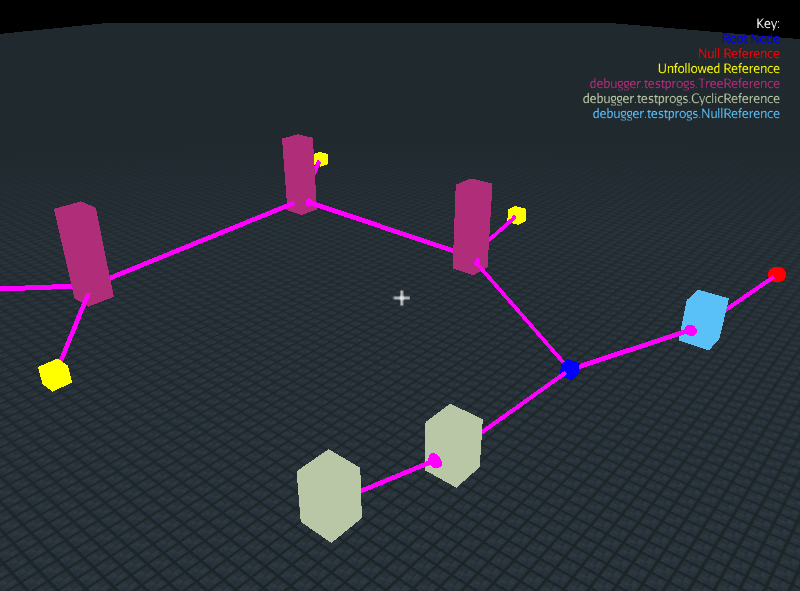
\includegraphics[width=0.75\textwidth]{images/final/random_colours.png}
        \caption{Coloured Types}
\end{figure}

References are represented by directed lines, this is represented by a line with a sphere attached where it meets the referenced object. There is a 1 to 1 mapping between objects on the heap and object vertices, so if an object is accessible via two different reference chains a cycle will be present in the graph.

\begin{figure}[h]
        \centering
        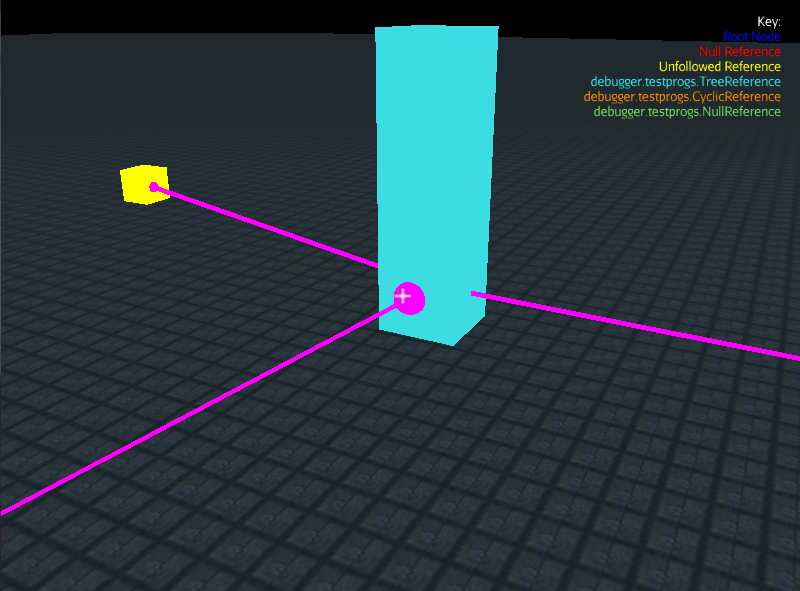
\includegraphics[width=0.75\textwidth]{images/final/directed_lines.png}
        \caption{Directed Lines}
\end{figure} 

The size of the space in which vertices in the graph exist is expanded dynamically as the number of objects in the graph grows.  The graph space is defined as a square with each side length proportional to the square root of the number of vertices in the graph. The aim here is to keep the density of vertices in the layout space constant even as unfollowed references are expanded and new vertices are added to the graph. As a result, VisualHeap can present both small and large graphs clearly.

\begin{figure}[h]
        \centering
        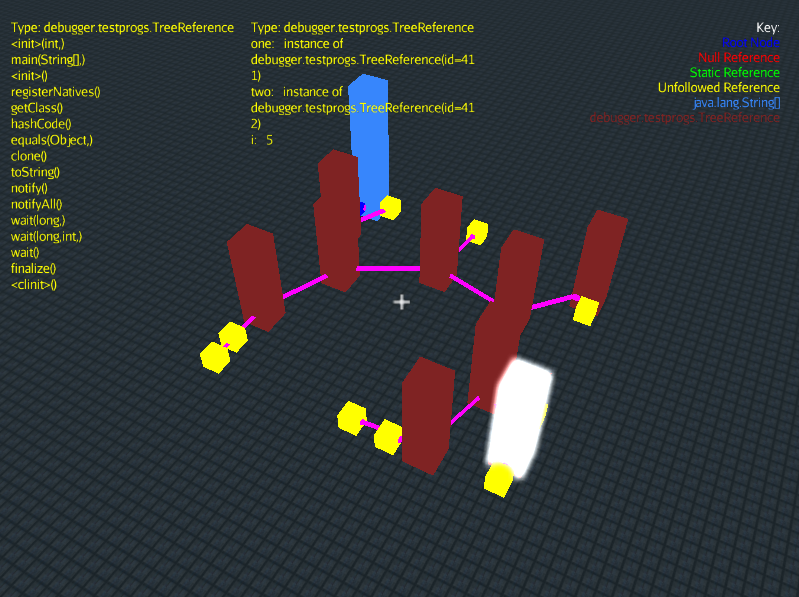
\includegraphics[width=0.75\textwidth]{images/final/dynamicoff.png}
        \caption{Object Selection}
\end{figure}

\subsection{Object Details}

The user can interact with the heap graph by clicking vertices. What kind of action results depends on the kind of object which is represented by the vertex.

Clicking an object vertex will display information about that object. This is done by acquiring the referenceType of the object and then printing out all it’s fields and their values. Selecting the stack frame/dummy vertex or a null reference will not reveal any useful information.

The user can request an unfollowed reference to be expanded by clicking the vertex representing it. When this happens, the unfollowed reference will be replaced with the appropriate type of vertex depending on whether it is an object or null reference and any children (fields) it has will be added as unfollowed vertices.

Due to the nature of our layout algorithm it is often easy to lose the expanded vertex after clicking on it. To combat this we also give any selected vertex an additional white glow to highlight it from the other vertices of the same type. In the future it would also be useful to be able to move the player to where the expanded vertex has been moved to upon the layout algorithm being rerun but within our time frame this was outside the scope of our project.

\subsection{Layout}

When selecting a layout algorithm (to assign 2D coordinates to each vertex in the graph), we identified 3 key requirements. The algorithm should produce visually appealing layouts; it should minimise the number of edges that are crossing and space vertices equally. Ideally, there should be some continuity between the layouts produced when a new vertex is added to a graph. Finally, the algorithm should be efficient. We tested 3 algorithms, Fructerman-Reingold (FR), an Inverted Self Organising Map (ISOM) and Kamada-Kawai (KK). These each had their own strengths, so we made the decision to provide all of them, with a default to ISOM.

\chapter{Implementation}

\section{Language}

We chose Java as our implementation language for this project. There were several key factors in making this decision. For us as a team, this was a good language choice as we are all experienced with Java. For the project, one of the most interesting reasons for choosing Java was so that we could run VisualHeap on itself, which we felt would be an intriguing test case for demonstrating our project’s capabilities. Furthermore, despite the fact that attaching to and inspecting a JVM is possible from many languages via the Java Virtual Machine Tools Interface, this is a low level interface. On the other hand the Java Debugger Interface is a higher level interface but is only available in Java. The JDI also had more clearly explained examples than any other interface, making it a more viable starting point for our project.

\section{Overview}

VisualHeap is split into three parts: a custom debugger (with GUI), a 2 dimensional graph layout builder and a 3D presentation engine.

The debugger controls a JVM running the program to be visualised. It also allows the layout builder to learn the object references held by a given object. The graph layout builder uses this service to build a graph of references between objects and produces a layout for this graph on a 2D plane. This layout is used to present the graph in the 3D engine.

Throughout our project we made use of the following frameworks and libraries:     
Java Debugger Interface (JDI), a high level debugger interface. Part of the Java Platform Debugger Architecture. Provided as standard by JVMs.
Java Unified Network / Graph Framework (JUNG), a framework with graph manipulation.
jMonkeyEngine (jME), a fully fledged 3D game engine written in Java.

\section{Debugger}

The debugger module of VisualHeap is built using the Java Debugger Interface, a high level interface provided by all JVMs as standard. The interface allows us to invoke Java programs, set breakpoints and step executing as well as inspect their memory.

The JDI uses an event based model. When certain conditions are reached in the child process (method calls, reaching a breakpoint), an event is generated and queued for the debugging process to receive. Filters can be added to cut down the number of events sent to the debugging process. The JDI allows breakpoints to be set and programs to be stepped by registering the appropriate Request with the client JVM.

We dealt with the asynchronous nature of this communication by creating an event thread which continuously polls the JDI event queue for new events of interest. When one of these occurs, information is passed out of the debugger module by calling the relevant callback function on an object implementing the DebugListener interface, where it is then handled appropriately by each listener.

One such listener was the graphical interface we present to the user, built using Java’s Swing library. The user can use the GUI to select a Java class to run (either from within a compiled package structure or a JAR file) and set breakpoints within that program. Once the program reaches a breakpoint, the user can click the “Visualise” button, which opens the 3D visualisation. In addition, the user can choose to step to the next point of execution or resume the program execution, until the next breakpoint, or the end of the program.

By listening to events received from the debugger module, it can update its own state to reflect the current state of the program. Thus, different parts of the interface are available based on a finite state machine.

\begin{figure}[h]
        \centering
        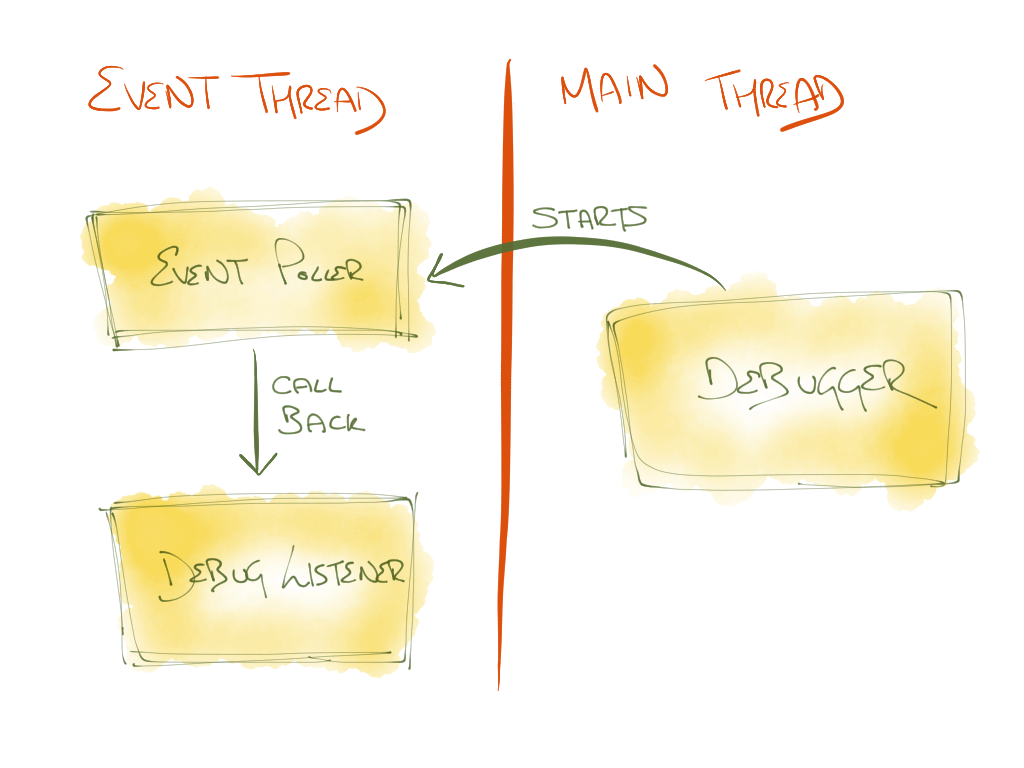
\includegraphics[width=0.75\textwidth]{images/final/thread.png}
        \caption{Threads}
\end{figure}

We chose this design because it is straightforward. The interactions between the main thread and event thread are very simple so the design suffices.

\section{Visualiser Module}

When a breakpoint is reached the debugger passes a list of the object references on the current stack frame to it’s registered DebugListener instance.

This list is given to the visualisation module via the GUI. We construct a graph of the heap with vertices representing objects and a directed edge between objects A and B iff one of A’s fields is a reference to B. Our algorithm is a straightforward recursive search limited to a depth of 3. Unexplored references are left to be expanded as the user requests.

We represent the graph using JUNG’s SparseDirectedGraph class, with instances of our own Vertex and Edge classes for the components, which allows us to use JUNG’s layout algorithms.

\begin{figure}[h]
        \centering
        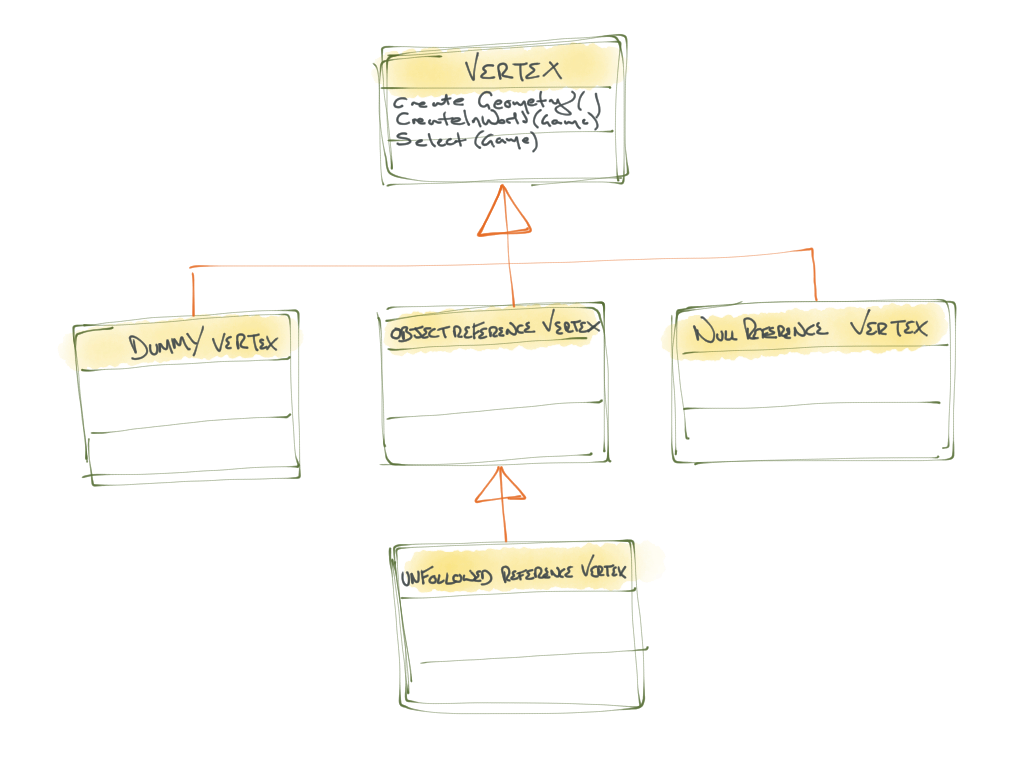
\includegraphics[width=0.75\textwidth]{images/final/vertex.png}
        \caption{Vertex UML}
\end{figure}

Different subclasses of the abstract Vertex class represent different types of vertices. A null reference is represented by an instance of the NullReferenceVertex class, an object reference by one of the ObjectReferenceVertex class. As how vertices should be represented in 3D space depends only on the object in memory that they represent, each subclass of Vertex implements methods to add itself to the world and perform an action when it is selected by the user.

\section{Producing a Layout}

In order to correctly denote the object within the program heap they must first be positioned as vertices of a graph and positioned within the 3D space we had created. Crucially they cannot simply be randomly positioned as the data must be organised and clear. With this in mind we have employed the use of the Java Universal Network/Graph Framework (JUNG) - a software library that provides a common and extensible library for the modelling and analysis of such graphs. JUNG is also written in Java and so applications that incorporate it are able to make use of the built-in Java API alongside other third party Java libraries. All layout algorithms implemented within JUNG are subclasses of the abstract Layout class which handles simple parameters such as the dimension size of the space and coordinates.

The first iteration of our product tested the Fruchterman-Reingold (FR) force-directed algorithm as implemented by JUNG. This worked well but after certain features did not operate as fully as we first hoped we tested a self-organising map, as implemented by JUNG, due to the similarity in the nature of the two algorithms. Both algorithms are discussed below to express the general intuition and formula of the algorithms, alongside product specific analysis; the algorithms will not be discussed in much greater depth than this as, whilst academically interesting, such detail is not relevant to the points of interest in this project.

\subsection{Force Directed}

The FR algorithm takes the difficult problem of drawing a graph and simplifies it by modelling as a physical simulation. The advantage of this is that no special knowledge of graph theory is required; the principle is intuitive.

Vertices are modelled as charged particles, with edges between them modelled as springs. A repulsive force exists between all pairs of vertices, analogous to the Coulomb force. Vertices linked by an edge have an attractive force between them, governed by Hooke’s Law. The layout is generated by moving vertices to minimise the energy of the system.

\begin{quote}

Coulomb’s Law, for our purposes: \\
$|F| \propto \frac{1}{r^2}$ where $r = distance between particles$.\\
Hooke’s Law : \\
$F = k x$, $k$ is stiffness, $x$ is extension.

\end{quote}

\begin{figure}[h]
        \centering
        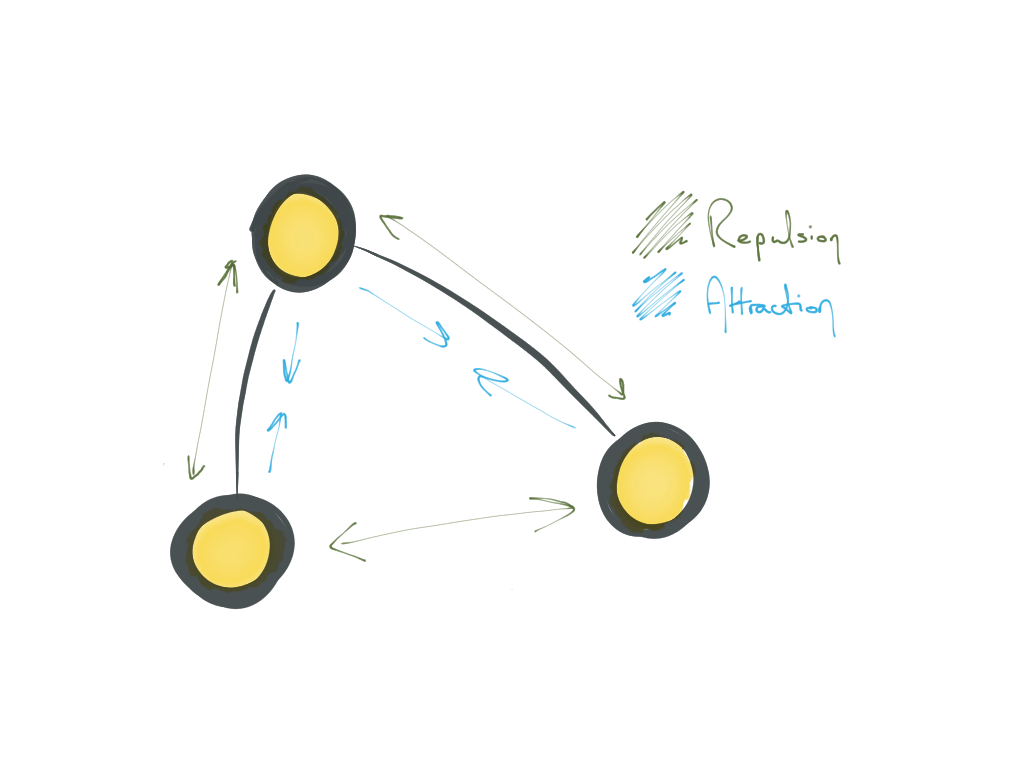
\includegraphics[width=0.75\textwidth]{images/final/frnodes.png}
        \caption{FR Node Layout}
\end{figure}

FR builds on this technique by adding an overall “temperature” to the system which governs step size (how far to move a vertex each iteration). Temperature decreases over time, ensuring the system stabilizes.

A disadvantage of this algorithm is that it makes no attempt to take advantage of planarity in the graph. This can lead to confusing layouts with edges crossing eachother. Also, it often gets stuck in local minima, leading to frustratingly poor layouts.

Another force-directed algorithm of interest was the Kamada-Kawai algorithm (KK) which focuses more on the uniform distribution of vertices rather than the least number of crossing edges; the balanced layout of vertices relate to the dynamically balanced spring system. This has similar problems to the FR algorithm in that it gets stuck in a local minima as the result is often influenced by the starting positions of the algorithm. Those interested in the planarity of a graph are less inclined to see KK as an attractive layout. Given our requirement for clarity when outlining the data structures provided to the system, KK has been included for completeness while utilising the JUNG framework. 

\subsection{Inverted Self Organising Maps}

The ISOM implementation in JUNG is based off of Meyer’s self-organising map algorithm, which in turn is an extension to Kohonen’s original self-organising map (SOM). This is a well established neural network type - a kind of unsupervised competitive network. This differs from the concept of supervised learning which requires a teacher and a priori objective function; instead the net discovers the object function itself. A given number of outputs compete with one another to be the ‘winner’ of a certain input signal - the winner is adapted to be a better fit for the signal. Given this is based on a Kohonen SOM there is only a single input layer and a single output layer; every unit in the competitive layer (the output layer) will be connected to an input layer. This scenario does not feature a biological aspect and so rather than focus on the response time between input and output it instead weights its learning function based on the weight space of the units.

\begin{figure}[h]
        \centering
        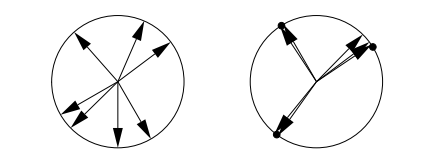
\includegraphics[width=0.3\textwidth]{images/final/weight.png}
        \caption{Updates in Weight Space}
\end{figure}

The weight set for each unit is represented as a vector and this vector is modelled using arrows. The network then solves a clustering task to align its weight vectors with input vectors it can see. By restricting this to two dimensions the weight vector can be easily translated as a position in 2D-space, enabling the network to be modelled as a graph. 

The difference between the original SOM and this ISOM implementation is in the interpretation of input and output. This implementation is so named the Inverted Self-Organising Map because it discards the actual network output and forms part of the original input as a fixed aspect of the algorithm.

ISOM ensures 1) a uniform filling of the space it is given and 2) that the graph-theoretic distance of all node pairs is matched with their metric distance. We may consider 1 as the repellent forces and 2 as the attractive forces and from here we may see how the objective of ISOM and FR are so similar. ISOM is often potentially faster than FR as it’s method allow it to eliminate the need to find a good heuristic procedure for finding the equilibrium between forces. ISOM is easily adaptable to many layout spaces as it can be more explicitly parameterized with its metrics. For our purposes ISOMs better results with planar graphs it was natural for us to move to this algorithm on our second iteration. It’s spread of nodes within the space was much more uniform, both with a fixed world size and a dynamically expanding one.

\begin{figure}[h]
        \centering
        \begin{subfigure}[b]{0.4\textwidth}
                \centering
                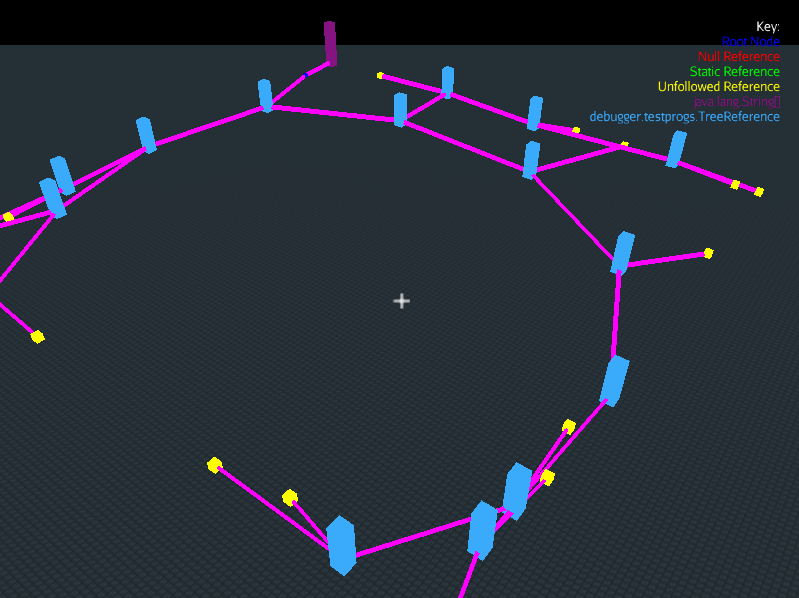
\includegraphics[width=\textwidth]{images/final/frcomparison.png}
                \caption{FR}
        \end{subfigure}%
        \qquad
        \begin{subfigure}[b]{0.4\textwidth}
                \centering
                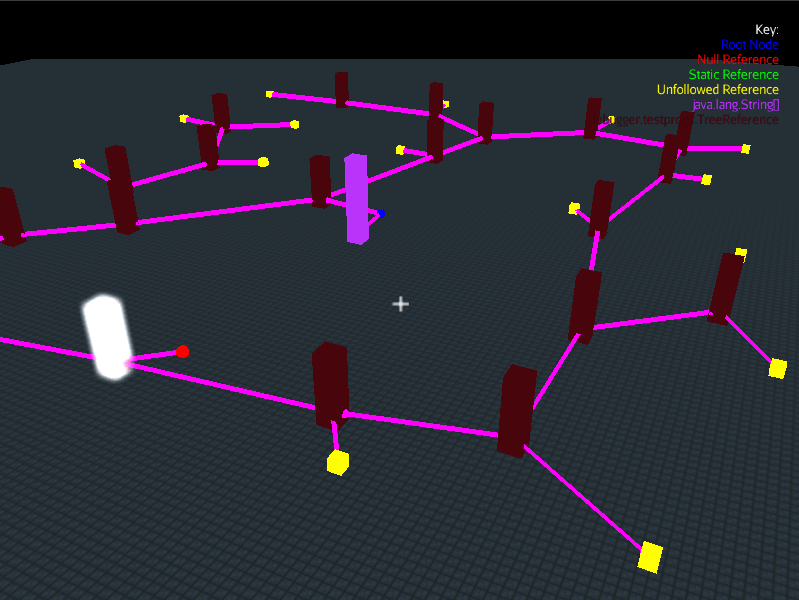
\includegraphics[width=\textwidth]{images/final/isomcomparison.png}
                \caption{ISOM}
        \end{subfigure}
        \qquad
        \begin{subfigure}[b]{0.4\textwidth}
                \centering
                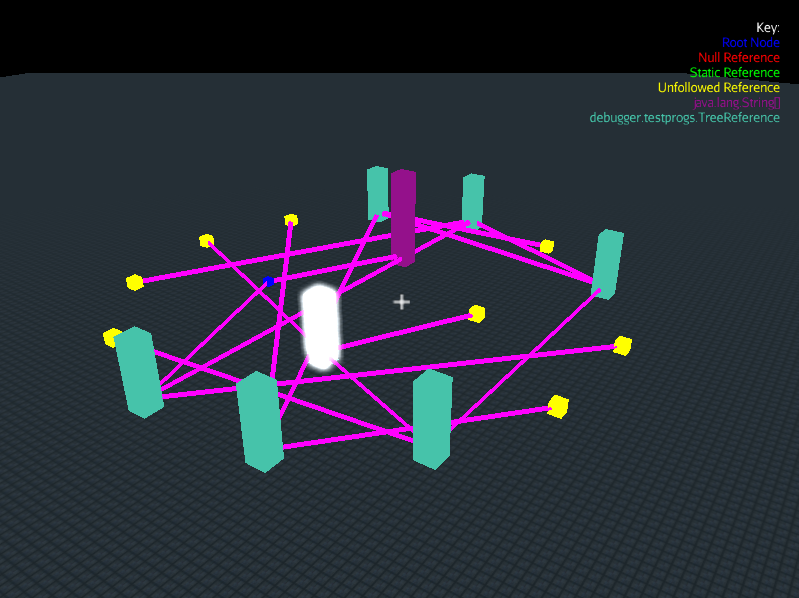
\includegraphics[width=\textwidth]{images/final/kkcomparison.png}
                \caption{KK}
        \end{subfigure}
        \caption{}\label{}
\end{figure}

\section{Graphics}

\subsection{Game Engine Selection}

The 3D rendering of the heap is the key component of VisualHeap so it was important to make the right implementation decision. We evaluated several methods of rendering the 3D world, including Java’s 3D API, the Unity C{\#}/Javascript engine and jme3. It was quickly realised that Unity would not integrate smoothly with our current work on the debugger and required us to learn new languages. We then aimed to find a 3D rendering method which could integrate with our debugger perfectly, preferably in java. The main drawback of Java 3D was that it was a heavyweight component, so it could have proved tricky to link together the windows of our java swing application with the 3D visualisation. Whilst not impossible, as there are workarounds for using them in the same containers, it will require extra thought to link things up as we require them. This said, it’s high-level, object oriented view of 3D graphics makes it straight forward to learn and as it is optimized for speed where possible it is a good fit for our application. We finally decided upon using the game engine JMonkeyEngine 3, which could be set up in Eclipse/Intellij and contained many libraries for rendering and mathematics making it simpler than using Java 3D. 

\subsection{Layout Update}

The vertices and edges of the graph are then drawn in the 3D space provided by jME3. A Vertex or Edge instance is registered with jME3 just after it is constructed.

\begin{figure}[h]
        \centering
        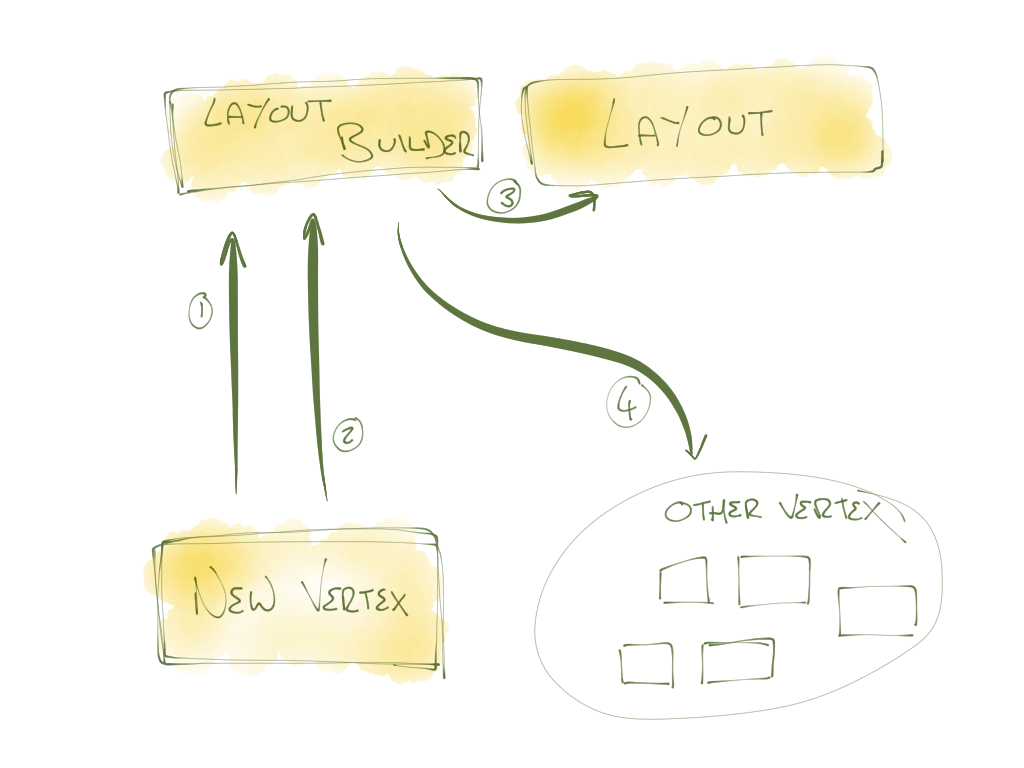
\includegraphics[width=0.75\textwidth]{images/final/builder.png}
        \caption{Layout Builder}
\end{figure}

\begin{enumerate}

  \item Register Creation
  \item Triggers Algorithm Execution
  \item Iterates Over Chosen Algorithm
  \item Update Current State

\end{enumerate}

When the layout is recomputed (i.e. after a new reference has been followed), we use an observer pattern to keep the positional information stored in Vertex and Edge instances up to date. These objects observe the Layout object. When the layout is changed they are notified, leading them to query the Layout for their new position. Using this information, they update jME3’s objects representing them to reflect their new location. This is much more efficient than the alternative of reconstructing the entire 3D representation as jME’s internal objects can be reused.

\subsection{Target Detection}
	 	 	 	 	
We applied ray casting algorithm on objects when an object is picked. The line(ray) casts from the camera into camera direction. Intersections between ray and all nodes are collected and the closest node is our target. This simple implementation let us to pick the right object and when clicked information of selected object is shown on screen. 

\chapter{Project Management}

This section aims to present the planning and project management techniques that we have used throughout the development stages of our product. We will cover the agile practices we have employed, continuous integration, planning and development tools and our roles within the group. 

\section{Planning}

We initially needed to come up with a list of requirements for the project so we could divide up the work. We did this using use case analysis, discussion with our supervisor and planning poker. We chose to implement use case analysis to structure our requirements process so we can first consider the requirements at a higher level using user stories, walk through a living scenario and then develop the specifications. After receiving feedback on our user stories from our supervisor, we morphed them into our final requirements and use cases. At the beginning of our project we were unsure which of the routes would be best to take our product: educational, gaming, professional use within industry. As we had a limited amount of time to develop we needed to make a decision so we could construct a requirements list. Each possible application had merits, but we decided on developing an educational tool mainly because we have all been in the situation where we didn’t understand how the heap worked or what was stored there and we know how useful a tool like this could have been when we were learning about it. Developing an educational tool also had the added benefit of being able to use our supervisor as a customer as he teaches first year students Java. Now we had a list of requirements we began planning how to achieve them. The first step was to play planning poker, since we intended on work in weekly sprints we decided to use planning poker to estimate how long each feature would take to implement. We then plotted these estimates on a gantt chart so we all had a visual representation of our targets.

\section{Agile Practices}

As we wanted our project to be developed in an agile environment we researched agile development before beginning our project to find ideas on how to become more productive. This is what encouraged us to use resources such as Trello and planning poker to ensure we would be working with an iterative approach as well as working in weekly sprints. We made using the agile development system a requirement as it promotes adaptive planning, evolutionary development and encourages rapid and flexible response to change.

\subsection{Stand-ups}

We adapted our weekly meetings to stand-ups to aid communication while not cutting into development time. Our stand-ups enabled us to be efficient and to the point as we discussed what we achieved that week, any issues we may be struggling with, any new ideas we have and what we hope to achieve the following week as well as allocating new tasks. In such as large group, communication is key to developing a sound system, so these stand ups were an important part of our agile development process. 

\subsection{Pair Programming}

Pair programming is a technique some consider quite integral to the extreme programming agile methodology.There is evidence which suggests that this produces a higher quality of code as it has been checked and discussed between two people, resulting in better design and readability, as well as fewer errors. By employing a collaborative approach to development we were able to  provide advice or alternative implementations and maintain communication to ensure we were all working towards the same requirements. 

We aimed to work in pairs as frequently as possible throughout the project, finding the results were more productive and resulted in a wider understanding of the area than working alone. At the beginning of each sprint we aimed to pair program to begin the new features. At the beginning of the next sprint, we swap partners so that one person from a pair will work on a completely different area, the other on a similar one. In this way, knowledge can be passed between us on every part of the system, which we believe is important to expand our learning.

\section{Trello}

Our group opted to managed our work predominantly through the project management website, trello.com. This is a useful website based on the kanban system, a scheduling system for just-in-time production. Trello allowed us to control the flow of development by assigning cards (representing features) to group members and the card would be moved along the board as it was developed (eg. moving a card from ‘to-do’ to ‘doing’). This system allowed us to keep track of exactly which tasks were assigned to each member of the group and how much of any given task had been completed. 

Keeping Trello up-to-date was key in each individual maintaining an understanding of where the project as a whole was at any given moment. Combining this with our weekly group meetings ensured everyone was up-to-date with the project and aware of what needed to be done. This was key in the development of our product so that if someone had an idea that wasn’t relevant to the section they were currently working on it could be communicated effectively to another group member.

\section{Version Control}

Version control is a fundamental feature of any software project. The main benefits of version  control arise in the face of loss and reverting changes in the case of bugs.

Using GitHub for storing our project was a very easy decision to make as we have all used its features before and we’ve found it very easy to use and integrate into previous projects. We opted to store and work within a private Git repository, allowing us to keep track of all the code provided by each member. Git's branching model allows users to have multiple local branches that can be entirely independent of each other. This is ideal for group project work as it will enable us to experiment with different ideas without fear of breaking existing features and losing previous work.

\subsection{Continuous Integration}
	 	 	 	 	
One way of reducing problems when many individuals are working on the same project is through continuous integration(CI). A CI server will check each push by an automated build and any tests failure will result in a failed build.

We have implemented this practice by running Travis CI. It is a CI server that can be easily installed and integrated with GitHub. When a build fails, Travis CI will send an email to the committee and the owner of the repository so that we can fix the code as early as possible.

\section{Test-driven development}

In developing the debugger, we employed TDD to ensure that we were consistently validating the correctness of our our software. We feel that TDD has lead to a more modularized, flexible, and extensible code base as it required us to think of the software in terms of small units that can be written and tested independently and integrated together later. This leads to smaller, more focused classes, looser coupling, and cleaner interfaces. The design of the debugger was complemented by the use of the TDD design pattern, however we felt that the implementation graphics and 3D visualisation would be impeded by having to write tests prior to development and chose a more visual approach. 

\section{Group Organisation}

We decided upon three main areas to begin our project as they could be initially developed in parallel, the custom debugger, heap analysis and generating a 3D world.

Eleanor acted as group leader throughout the project, so she became responsible for CATE submissions, organising our weekly group meetings with the supervisor and settling the few disagreements between members.

Aviv and Oli began the project working on the debugger as they had the most experience in this area and we were keen to set the project off with a quick start. Anna and Eleanor started looking at heap analysis to discover what information could be gained to eventually use in the final product, this naturally lead on to also researching how best to present the layout of the graph produced. Briony and Ying were in charge of finding a 3D graphics engine to draw the visualisation to as they were keen to investigate various game engines and other options.

\chapter{Evaluation}

\section{Testing Procedures}

We used jUnit and jMock to write a suite of unit tests as we developed VisualHeap. Using the Java plugin for gradle makes integration with jUnit very straightforward; we were furnished with a full test report in HTML format each time the project was built.

\begin{figure}[h]
        \centering
        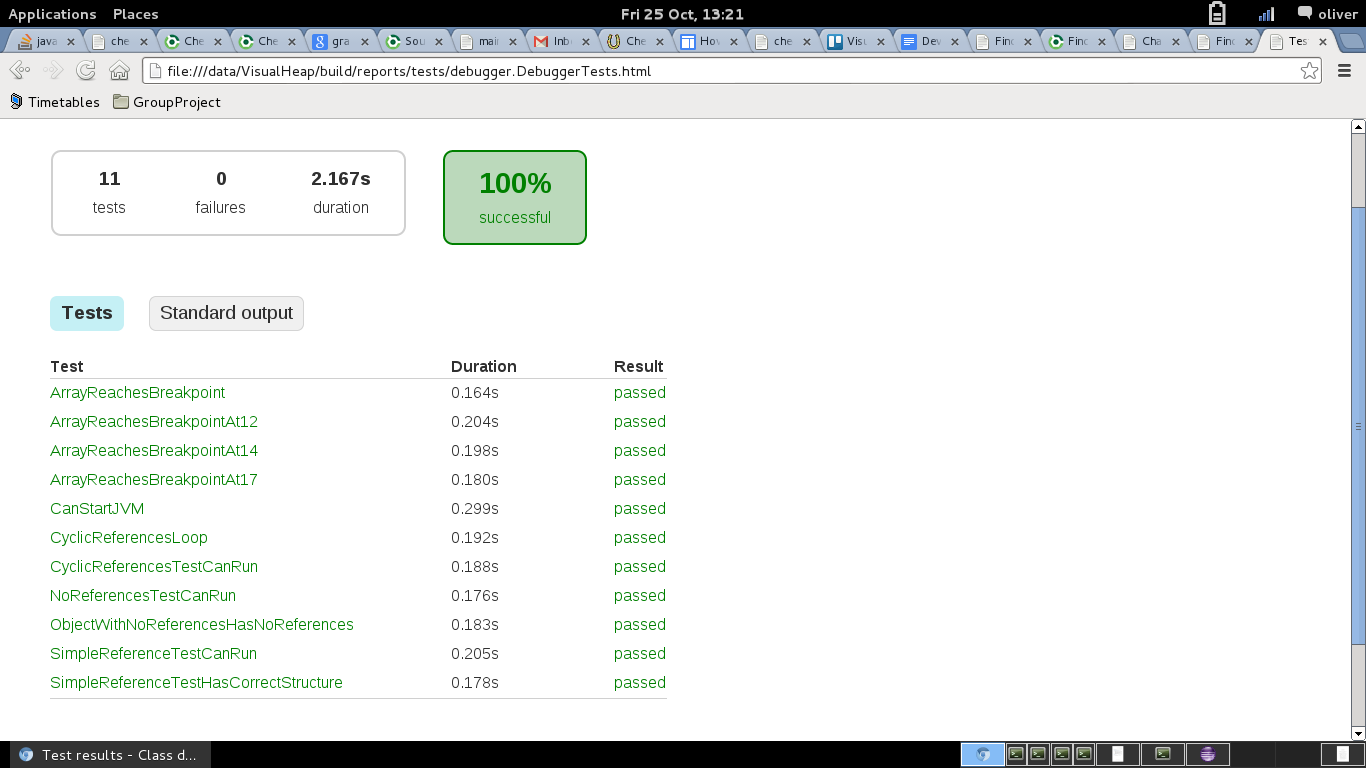
\includegraphics[width=0.75\textwidth]{images/final/testresults.png}
        \caption{HTML Test Report}
\end{figure}

When the project reached the stage of needing to see the visual output to debug and improve the program we opted to create multiple self-defined test cases to see how the program displayed a variety of programs. These tests included trees, simple references, cyclic references and tests containing many different data structures. This was important while we were developing the layout algorithm so we could see how many different objects would be displayed.

Once we were mainly using self-defined test cases we found it was quite time consuming to always enter the classpath of each test each time you ran the program. For this reason we set up the program to accept arguments for the classpath and qualified class name so we could run various tests more easily.

An interesting test case was running the tool on itself. The ability to do this was one of the main reasons we decided to write VisualHeap in Java. It also serves as the test of running VisualHeap on a much larger program than in our other test cases. This test did show that our application does not work that well on multi-threaded apps for the purposes of debugging. This is mostly due to time constraints preventing us from providing a useful interface for accommodating multi-threaded applications; they can still be visualised by VisualHeap.

\chapter{Challenges}

\section{Development Challenges}

\begin{itemize}
  \item Debugger
\end{itemize}

We experienced a few problems initially with learning to use the JDI as it requires a few specific bits of set up in order to work. It requires an understanding of Java class paths and linking which can be very difficult to configure correctly. This initial configuration has been simplified for the user as much as we can through the design of our GUI and in the fact that our final application is distributable stand-alone as a JAR file, further reducing the amount of setup required from the user.

When we started the project and determined that we wanted to use the Java Debugger Interface (JDI), we realised that while it has a very good set of API documentation for the individual classes involved in the interface, there were very few guides on how it all fits together to allow someone to construct an application from it. The best we had to go on were a few standard examples that come with the JDI library, which is where the very core of our debugger has been built upon.

\begin{itemize}
  \item Time Management
\end{itemize}

Due to a variety of work schedules and many group members taking different modules we initially found beginning the project difficult. Also due to the fact that certain parts of the project, such as generating the graph, were dependant on the debugger being functional it was difficult to split the project up into sections that we could all work on concurrently. However once the debugger was functional we were able to more readily split up tasks and our progress increased substantially.

Towards the end of the project we experiences minor difficulties communicating what needed to be done as many group members went on holiday or were unavailable to communicate with over Christmas. However we succeeded in completing the project on time as we agreed to all set aside a week where we would all be available to work on the project together.

\begin{itemize}
  \item Sensible Graph Layouts
\end{itemize}

Our initial choice of layout algorithm, Fruchterman-Reingold, failed to produce adequate layouts for the reference graph. New vertices would get trapped in corners or between other vertices. We first tried dynamically expanding world space as more vertices were added, but even then the algorithm would get stuck in local minima and not make full use of the the space available. 

The Self-Organising Map proved to make better use of the space available with the slightly better weight with respect to the connecting edges in the graph. The notable issue with this algorithm was that on following an unfollowed reference every vertex in the graph was liable to reposition itself. Whilst usually clearly laid out this made it very difficult to follow which node had been selected. This was dealt with by highlighting the selected vertex, initially with a glow on the object selected but when this proved difficult to see on darker colours so this was adapted during the second iteration to be a pure white glow on selection. White proved to always stand out against the other colours in use, especially when this colour was added into the hash map used to stop this colour being used as a type colour.

\begin{figure}[h]
        \centering
        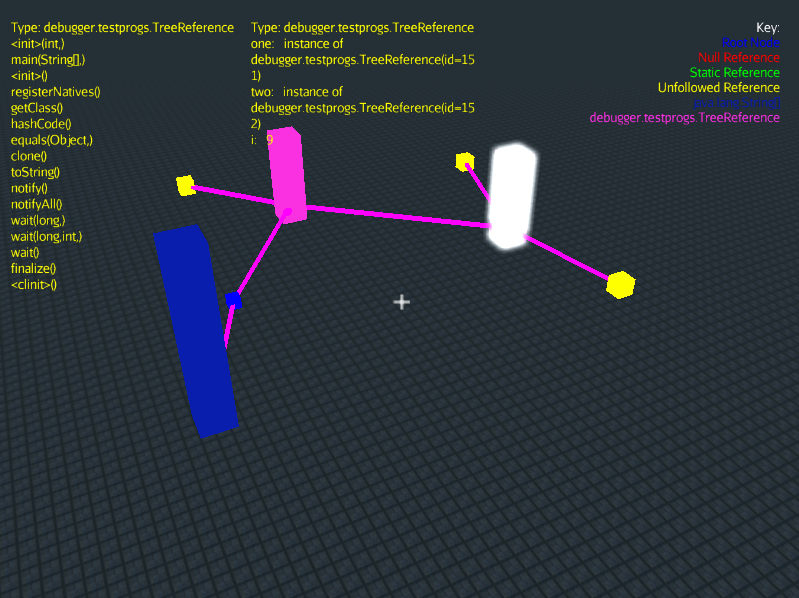
\includegraphics[width=0.75\textwidth]{images/final/objectselect.png}
        \caption{Object Selection}
\end{figure}

\begin{itemize}
  \item Presenting Object Information
\end{itemize}

As mentioned previously in the design section, on clicking an object we display information about that object. We encountered the challenge of deciding where to display this information and how to format it. Our initial thoughts were that it needed to be within the visualisation window so that a user would easily see information appearing when they clicked an object. However this provided one specific problem, what would happen if the object had too many fields or methods to display? 

Unfortunately for us the solution to this problem would be to either move the information into the GUI or to merge and recreate the GUI and visualisation screen using Nifty GUI. Either of these solutions would allow us to create scrollable text boxes to display the information in. Moving the information into the current GUI would mean the user may not notice when new information was being displayed as it would be much less obvious to display it away from the visualisation screen, so we decided this was not an effective solution. That left integrating the GUI and visualisation screen using Nifty GUI, however due to the time constraints of our project we were unable to complete this and so this is still a known issue.

\begin{itemize}
  \item Object Representation
\end{itemize}

We encountered the challenge of deciding how to represent different objects in our world. We had many initial ideas, some of which were quite excessive and would not have been achieved in our given time frame such as creating tunnels for references with hidden rooms for each object or making the graph plot points in 3 dimensions so we could create a universe where each planet or star was an object. However we knew we had a time limit so had to come up with a reasonable solution that still effectively conveyed all the important information to the user.

As the type and size of an object were the main points we wanted a user to be able to see from a glance we opted to display each type as a separate colour and the size was generated based on the number of fields an object had. We also created a key to allow a user to be able to see the type of an object easily. This is covered in more detail in the design section. 

\section{Feedback}

We had several group meetings with our supervisor throughout the duration of the project. In these sessions we would often gain feedback on the product and brainstorm new ideas for the next sprint. For example, we went through several re-factorings of the GUI and 3D world based on feedback from these meetings. We believe these meetings have helped us create a useful product that meets the initial criteria.

\section{Known Issues}

\begin{itemize}
  \item If number of object fields, methods or keys gets too large some are not viewable on the screen
\end{itemize}

As previously mentioned in challenges we were unable to implement scrollable text boxes to display the object information in without re-implementing parts of the project.

\begin{itemize}
  \item There is currently no mechanism for debugging in multiple threads
\end{itemize}

Breakpoints can be placed in code that executes in multiple threads, but we provide no tools for managing the exploration of heap usage in different threads.  As VisualHeap is primarily an educational tool for new programmers who won’t be interested in concurrency, we do not think this is a serious issue.

\begin{itemize}
  \item Breakpoints can’t be set easily inside anonymous inner classes, as these are wrapped in their own class files during compilation
\end{itemize}

\chapter{Future Extensions}

We had many different ideas for where we could take this project when we started out, however it would have been impossible to complete all of them in the given time frame. We will outline a few ideas here which could be implemented as extensions.

\begin{itemize}
  \item Tagging objects
\end{itemize}

While in the visualised world the user could physically interact with the objects by adding notes to the objects which would then be written on the object for later reference by the user. This interaction could also be used to allow the user to learn about garbage collection. A user would tag an object they thought would be garbage collected then the program would continue to run and they could find out if they were correct. This could also be implemented so a user could set certain objects to be garbage collected and see how that affected the program.

\begin{itemize}
  \item GUI Tooltips
\end{itemize}

Adding tooltips to the GUI to explain what each section does to first time users would be a very useful feature as our tool is targeted at new programming students who may not understand how breakpoints or debuggers work. These could be implemented so if a user hovered over a button in the GUI it would display a brief explanation of how to use it.

\begin{itemize}
  \item Stepping within debugger, show objects that have been garbage collected
\end{itemize}

Currently a program can be visualised multiple times during its execution but there is no continuity between what is shown. An interesting extension would be persistent objects between visualisations, allowing the user to accumulate a set of objects they are interested in and see how these are modified as the program executes. In the same vein, the ability to step whilst inside the visualiser and see how that changes the object graph would be a useful teaching tool.

\begin{itemize}
  \item Improved presentation of object details / NiftyGUI
\end{itemize}

At the moment when an object is clicked we present a listing of all the fields and types of the object, and then a list of each method the object contains. At the moment, if an object contains a large amount of either, the list will run off of the visualiser’s display window as there was no time to implement a scrollable or hidable panels to show the data within. With more time we could have looked into the Nifty GUI to implement some of these options within jME.

\begin{itemize}
  \item Alternative representation of common library objects, such as Arrays, Lists and Strings
\end{itemize}

Alternative representations for certain objects could provide additional teaching aids. As arrays, lists and strings are very common data structures they could be represented uniquely in the world so they were immediately recognisable by the user. For example, a string could be represented by a 3D representation of its first 5 letters. Or arrays could be presented as longer rectangles split into cells for each element, with lines representing object references coming out of the appropriate cell. The main difficulty in doing this would be extending the layout algorithms to take into account the dimensions of the vertex; a non trivial issue. Implementing these unique features would serve in making the world much more interesting for a user to look at and navigate around.

\begin{itemize}
  \item Layout
\end{itemize}

Further improvements could be made to the layout algorithm. Using the ISOM algorithm means that adding a new vertex results in a completely different graph layout. Alternative approaches we have not explored include extracting sub-graphs, producing a locally optimal layout and merging these for the entire graph. Another possibility is to return to using the more intuitive F-R layout algorithm when an unfollowed reference is expanded. When the graph layout becomes too difficult to follow, the user could click a ``panic button'' which runs the ISOM layout algorithm and produces a completely different but more pleasing layout.

\chapter{Conclusion}

In this section we will consider the task that was set to us by our supervisor and explain how we believe we have achieved it. The description of our task was set as follows:

\emph{``In this rather experimental project, we will design a tool which supports visualisation of the heap of a running Java program as a 3D scene which can be navigated by the software developer by moving around as if in a first person shooter game…''}

We have created a tool which allows a user to generate a 3D visualisation of the heap of a running Java program. It allows the user to move around the 3D world using similar controls to a first person shooter while also allowing a user to fly above the generated graph to gain a birds eye view of the scene. 

\emph{``...The project would involve integrating with a Java debugger so that, on reaching a program breakpoint, the contents of the heap is analysed and rendered on demand using a package for 3D modelling (perhaps a game engine)...''}

We have created our own micro-debugger using the standard Java Debugger Interface which allows us to set breakpoints and the data retrieved from this can be used to analyse objects on the heap in a 3D game engine on demand.

VisualHeap analyses the heap and displays a graphical representation of objects living there. They are joined by the references between the objects allowing a user to gain an understanding of how objects on the heap are connected. This visual representation can be obtained from any valid breakpoint in a Java program.

\emph{``...Because the heap of a Java program can be very large it will not be feasible to take a snapshot of the whole heap. Instead, the immediately visible portion of the heap, starting from the stack and static data, will be rendered, and additional data will be brought into play as the user walks through the heap world.''}

In our tool we incrementally explore the heap, initially to a depth of three beginning at the stack frame in which the breakpoint has occurred. To view additional data the user can request more data by clicking on an unfollowed reference to expand it. This adds new objects to the world and also changes the layout of the graph due to the layout algorithm we used. The expanded object is highlighted with a white glow to allow the user to locate the node they just expanded easily.

So based on these points we have met our original brief and produced a tool which meets our objective. This can then be used to improve the teaching of object oriented languages and memory management of future groups of students. 

\begin{appendices}

\chapter{Program Walkthrough}

\begin{figure}[h]
        \centering
        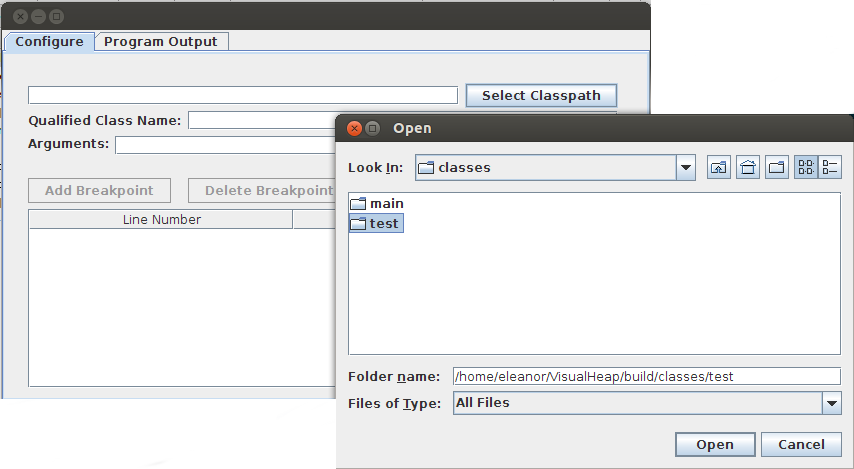
\includegraphics[width=0.75\textwidth]{images/final/walk1.png}
        \caption{Select Classpath}
\end{figure}

\begin{figure}[h]
        \centering
        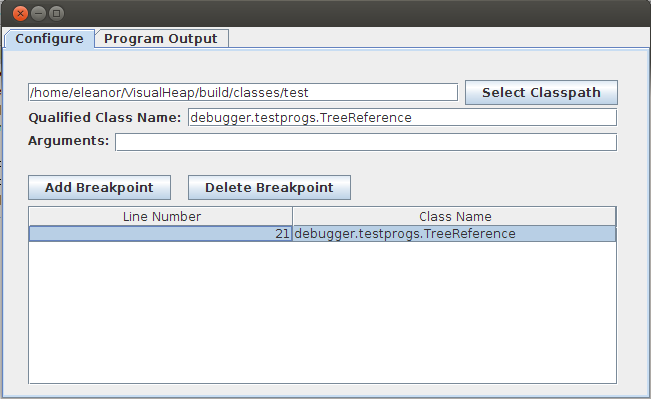
\includegraphics[width=0.75\textwidth]{images/final/walk2.png}
        \caption{Choose Program and Breakpoint}
\end{figure}

\begin{figure}[h]
        \centering
        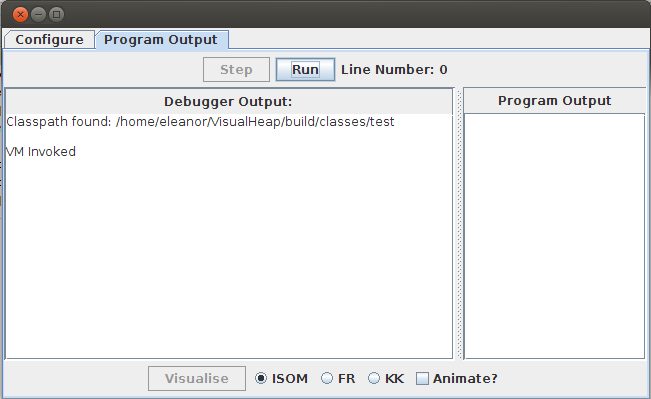
\includegraphics[width=0.75\textwidth]{images/final/walk3.png}
        \caption{Run Program}
\end{figure}

\begin{figure}[h]
        \centering
        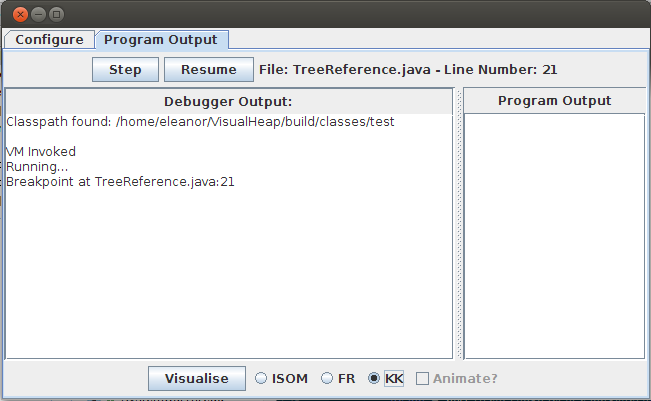
\includegraphics[width=0.75\textwidth]{images/final/walk4.png}
        \caption{Select Algorithm Layout}
\end{figure}

\begin{figure}[h]
        \centering
        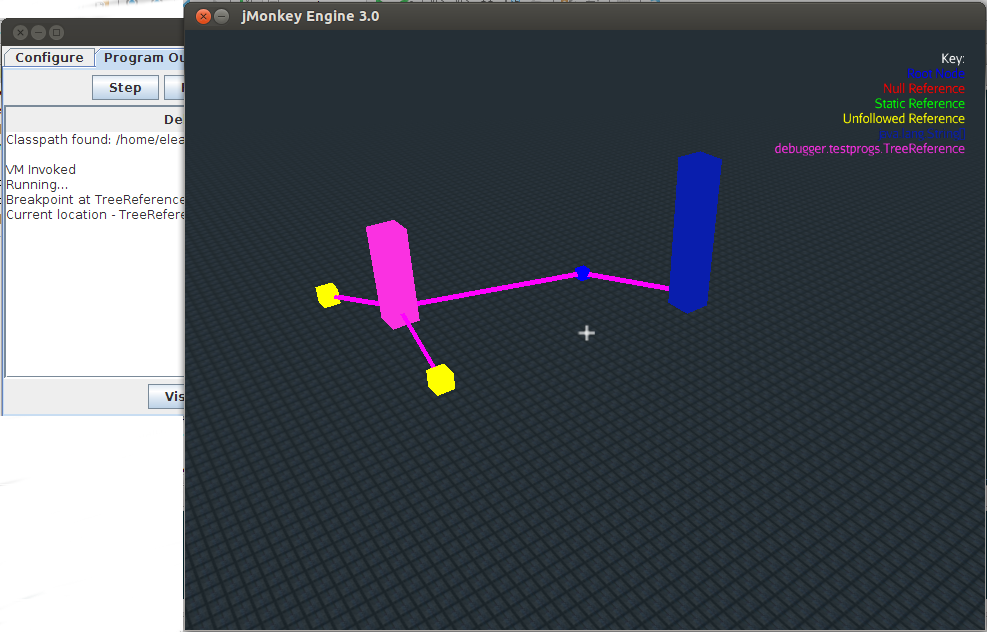
\includegraphics[width=0.75\textwidth]{images/final/walk5.png}
        \caption{Visualise}
\end{figure}

\end{appendices}

\begin{thebibliography}{9}

\bibitem{1}
  Bernd Meyer. 
  \\ \emph{Self-organizing graphs: A neural network perspective of graph layout. In Graph Drawing (GD'98)}, 
  \\Montreal, Canada, 
  \\August 1998

\bibitem{2}
  Fruchterman and Reingold, 
  \emph{Graph Drawing by Force-directed Placement}
 
\bibitem{3}
  GCspy,
  \\http://www.cs.kent.ac.uk/projects/gc/gcspy/

\bibitem{4}
  JDI, 
  \\http://docs.oracle.com/javase/7/docs/jdk/api/jpda/jdi/

\bibitem{5}
  Heuristic Evaluation,
  \\http://www.nngroup.com/articles/ten-usability-heuristics/
  
\bibitem{6}
  HeapViz,
  \\http://www.cs.tufts.edu/research/redline/heapviz/

\bibitem{7}
  Travis,
  \\https://travis-ci.org/

\bibitem{8}
  Jung,
  \\http://jung.sourceforge.net/

\bibitem{9}
  Gradle,
  \\http://www.gradle.org/

\bibitem{10}
  jME,
  \\http://jmonkeyengine.org/

\end{thebibliography}

\end{document}
